
\chapter{Persamaan Diferensial Biasa}
\begin{flushright}
\begin{tabular}{>{\centering}p{5cm}>{\raggedright}p{5cm}}
\multicolumn{2}{>{\raggedleft}p{10cm}}{\textit{Gerbang dan kunci menuju ilmu pengetahuan adalah matematika.}}\tabularnewline
$\ $ & --Roger Bacon (\textit{Opus Majus)}\tabularnewline
\end{tabular}
\par\end{flushright}

\begin{flushright}
\bigskip{}
\par\end{flushright}

\begin{flushright}
\begin{tabular}{>{\centering}p{5cm}>{\raggedright}p{5cm}}
\multicolumn{2}{>{\raggedleft}p{10cm}}{\textit{Seandainya saya memulai kembali studi saya, saya akan mengikuti
nasihat Plato dan memulainya dengan matematika.}}\tabularnewline
$\ $ & --Galileo Galilei\tabularnewline
\end{tabular}
\par\end{flushright}

\begin{flushright}
\bigskip{}
\par\end{flushright}

\section{\label{sec:OdePendulum}Gerak Bandul\index{bandul}}

\subsection{Sejarah singkat\index{bandul}}

Christiaan Huygens\index{Huygens, Christiaan} (1629-1695) dianggap
sebagai penemu jam bandul pada tahun 1656, sedangkan Galileo\index{Galileo}
Galilei (1564-1642) dianggap sebagai orang pertama yang melakukan
kajian ilmiah terhadap sifat-sifat bandul.\cite{naylor,scienceuk}
Dalam sebuah surat terkenal kepada Guidobaldo del Monte pada tahun
1602, Galileo menyatakan bahwa periode ayunan suatu bandul (waktu
yang dibutuhkan untuk berayun ke satu arah lalu kembali) tidak bergantung
pada amplitudo ayunan (seberapa jauh bandul berayun ke kiri dan kanan).
Del Monte menyanggahnya dengan menunjukkan bahwa bukti fisik tidak
mendukung pernyataan tersebut.\cite{matthews} Dan ia benar---bukti
fisik memang tidak mendukungnya; pernyataan Galileo sebenarnya keliru.
Periode sebuah bandul berubah menurut amplitudo ayunannya (jika semua
faktor lain tetap sama). 

Para sejarawan pada umumnya bersedia memaafkan Galileo atas kekeliruan
ini, mungkin antara lain karena periode bandul hampir konstan pada
amplitudo kecil, dan juga karena Galileo\index{Galileo} merupakan
tokoh utama dalam revolusi ilmiah (kelahiran ilmu pengetahuan modern)
pada abad ke-17. Temuannya mengenai gerak bandul hanyalah sebagian
kecil dari seluruh sumbangsihnya terhadap ilmu pengetahuan. Cara ia
memanfaatkan model matematis ideal dari dunia fisik untuk mendasari
pernyataan dan eksperimennya, suatu metode kajian ilmiah yang secara
langsung bertentangan dengan pandangan umum pada zamannya, menjadi
dasar revolusi ilmiah dan karena itu sekurang-kurangnya sama pentingnya
bagi ilmu pengetahuan dengan setiap penemuan ilmiahnya. Mengenai bandul,
ia memulai penyelidikan yang kelak (beberapa tahun setelah wafatnya)
menghasilkan metode untuk menentukan garis bujur di laut, suatu pencapaian
yang akan mengubah dunia! Dengan kemampuan menghitung garis bujur,
para pelaut dapat mengarungi lautan, menemukan tempat-tempat baru,
dan memetakan dunia. Dampak terbesarnya mungkin adalah kolonisasi
Eropa atas wilayah-wilayah asing.

Saat ini, ketika membayangkan bandul\index{bandul} yang kemungkinan
besar terlintas dalam benak kita adalah jam lantai. Walaupun dapat
dikatakan kurang penting dibandingkan sumbangsihnya bagi ilmu pengetahuan
dan navigasi, ketepatan pencatatan waktu yang dihadirkan jam bandul
membawa dampak besar bagi masyarakat luas. Berkat pencatatan waktu
yang akurat, kerja berbasis waktu, jadwal angkutan dan perdagangan,
waktu mulai yang diumumkan untuk ibadah atau pertemuan lain, serta
setiap gejala lain berbasis jam yang kini kita anggap biasa menjadi
mungkin. Pada abad ke-17, semua ini merupakan hal baru. Untuk memberi
gambaran tentang betapa pentingnya jam, dan dengan demikian bandul,
bagi masyarakat, pertimbangkan pernyataan Mumford: ``jam, bukan mesin
uap, adalah mesin utama zaman industri modern.''\cite{mumford} 

\noindent\begin{digression}{Jam Bandul}

\noindent Galileo\index{Galileo} tidak pernah menerapkan bandul\index{bandul}
sebagai mekanisme pencatatan waktu. Baru sekitar 15 tahun setelah
Galileo wafat, jam bandul menjadi kenyataan. Walaupun jam bandul pertamanya
(1656) lebih akurat daripada jam lain mana pun pada saat itu, Huygens\index{Huygens, Christiaan}
berupaya menyempurnakan rancangannya. Dalam upayanya, ia membangun
sebuah jam dengan bandul yang dimodifikasi dan menerbitkan karya klasik,
\textit{Horologium Oscillatorium}, yang untuk pertama kalinya memaparkan
rincian matematis mengenai isokronisme sikloid, pada tahun 1673.\cite{scienceuk,tsbts} 

Saat ini kita menerima begitu saja bahwa sikloid adalah lintasan yang
harus diikuti benda jatuh agar perjalanannya menuju suatu titik berlangsung
dalam waktu yang sama, terlepas dari posisi awalnya. Kita juga menerima
begitu saja bahwa periode sebuah bandul sederhana berubah menurut
amplitudonya. Kita memiliki lebih dari 400 tahun wawasan fisika dan
matematika yang memberi tahu kita demikian! 

\noindent\end{digression}

\subsection{Persamaan gerak\index{bandul}}

Setelah mudah-mudahan berhasil menjelaskan mengapa bandul menarik
untuk dikaji, mari kita beralih ke penurunan modern gerak bandul dengan
menggunakan diagram benda bebas\index{diagram benda bebas}, salah
satu perangkat utama dalam teknik mesin. Dalam diagram benda bebas,
sebuah benda, dalam hal ini beban bandul, diisolasi dari segala sesuatu
kecuali gaya-gaya yang bekerja padanya. Gaya-gaya tersebut ditunjukkan
dengan vektor, lalu hukum gerak kedua Newton\index{Newton!hukum gerak kedua}
(percepatan suatu benda berbanding lurus dengan besar gaya resultan
yang diberikan pada benda itu, searah dengan gaya resultan, dan berbanding
terbalik dengan massa benda, atau $F=ma$) diterapkan.
\begin{figure}
\caption{\label{fig:Free-body-diagram}Diagram benda bebas untuk sebuah bandul.}

\centering{}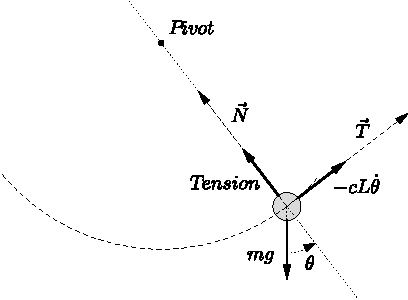
\includegraphics{figures/ode-pendulum01}
\end{figure}
Gambar \ref{fig:Free-body-diagram} menunjukkan tiga gaya yang bekerja
pada sebuah bandul---gaya gravitasi\index{gaya!gravitasi}; tegangan\index{gaya!tegangan}
pada batang atau tali yang menahan beban pada titik tumpu; dan gaya
ketiga yang disebut gaya hambat\index{gaya!hambat}, yang timbul akibat
hambatan udara---beserta arah normal ($\vec{N}$) dan tangensial
($\vec{T}$) terhadap lintasan bandul. Secara teknis, hanya beban
bandul dan ketiga gaya tersebut yang merupakan bagian dari diagram
benda bebas. Unsur lain bukan bagian dari diagram benda bebas, tetapi
ditambahkan dengan garis putus-putus untuk membantu menjelaskan gerak.
Panjang bandul dianggap $\ell$, dan kita akan menerapkan hukum kedua
Newton dalam arah tangensial terhadap gerak, yaitu arah $\vec{T}$.

Kelajuan beban bandul adalah hasil kali panjang bandul dan kecepatan
sudut, $\ell\dot{\theta}$. Percepatan beban bandul, yaitu turunan
kelajuan, adalah $\frac{d}{dt}\left(\ell\dot{\theta}\right)=\ell\ddot{\theta}$.
Oleh karena itu, suku $ma$ (massa dikalikan percepatan) dalam hukum
kedua Newton untuk gerak sebuah bandul\index{bandul} adalah $ml\ddot{\theta}$.

Gravitasi\index{gaya!gravitasi} menimbulkan gaya tetap yang arahnya
ke bawah pada beban bandul, dengan besar yang sama dengan berat beban,
$mg$. Namun, besar gaya ini dalam arah $\vec{T}$ adalah $mg\sin\theta$.
Ada baiknya kita berhenti sejenak untuk memastikan tandanya benar.
Untuk nilai $\theta$ antara 0 dan $\pi$, beban berada di sebelah
kanan titik tumpu, sehingga gaya gravitasi cenderung mempercepat beban
searah jarum jam (negatif terhadap $\theta$). Karena $mg\sin\theta$
positif untuk nilai $\theta$ antara 0 dan $\pi$, gaya akibat gravitasi
sebenarnya adalah $-mg\sin\theta$. Untuk nilai $\theta$ antara $-\pi$
dan 0, beban berada di sebelah kiri titik tumpu, sehingga gaya gravitasi
cenderung mempercepat beban berlawanan arah jarum jam (positif terhadap
$\theta$). Karena $mg\sin\theta$ negatif untuk nilai $\theta$ antara
$-\pi$ dan 0, gaya akibat gravitasi kembali bernilai $-mg\sin\theta$.
Analisis serupa untuk sudut lain akan memberikan kesimpulan yang sama.

Gaya redaman atau gaya hambat (hambatan udara)\index{gaya!hambat}
dianggap sebagai gaya yang sebanding dengan kelajuan beban bandul,
$\ell\dot{\theta}$, sehingga besarnya $c\ell\dot{\theta}$. Gaya
redaman selalu dianggap melawan gerak secara langsung, sehingga seluruh
gaya redaman berada dalam arah $\vec{T}$. Tinggal memilih tanda yang
benar. Karena $\dot{\theta}$ menunjukkan arah gerak, gaya redaman
harus bertanda sebaliknya. Konstanta redaman $c$ dianggap positif,
dan tentu saja $\ell$ positif, sehingga gaya redaman harus $-c\ell\dot{\theta}$.

Tegangan\index{gaya!tegangan} yang bekerja pada beban bandul tidak
relevan karena selalu tegak lurus terhadap gerak. Komponen tegangan
dalam arah tangensial selalu nol.

Dengan mengganti $F$ dengan jumlah gaya tangensial tersebut, hukum
kedua Newton yang diterapkan pada bandul menjadi $-mg\sin\theta-c\ell\dot{\theta}-0=m\ell\ddot{\theta}$
atau
\begin{equation}
\ddot{\theta}+\frac{c}{m}\dot{\theta}+\frac{g}{\ell}\sin\theta=0.\label{eq:pendulum}
\end{equation}
Persamaan \ref{eq:pendulum} dikenal sebagai persamaan diferensial\index{persamaan diferensial}
karena merupakan persamaan yang melibatkan turunan (atau diferensial).
Lebih tepatnya, persamaan tersebut merupakan persamaan diferensial
biasa berderajat dua\index{persamaan diferensial!biasa} (PDB)\index{PDB|see{persamaan diferensial, biasa}}.
Berderajat dua\index{persamaan diferensial!derajat} karena derajat
turunan tertingginya adalah dua, dan biasa karena hanya melibatkan
satu variabel bebas (waktu $t$).\index{bandul}

Persamaan diferensial paling sederhana dipelajari dalam kalkulus,
meskipun istilah ``persamaan diferensial'' jarang digunakan. Ketika
pertama kali membahas gagasan antidiferensiasi, pertanyaan ``Fungsi
apa yang turunannya sama dengan ...?'' pasti muncul. Sebagai contoh,
kita mungkin dihadapkan pada pertanyaan: fungsi apa yang turunannya
sama dengan $x$? Pertanyaan ini juga dapat diajukan sebagai: fungsi
$y$ apa yang memenuhi persamaan (diferensial) $y'=x$? Jawabannya
dapat diperoleh dengan mengintegralkan persamaan tersebut:
\begin{eqnarray*}
\int y'\,dx & = & \int x\,dx\\
y & = & \frac{1}{2}x^{2}+C
\end{eqnarray*}
 (jangan lupakan konstanta integrasi!).

\subsection{Gaya-gaya dalam diagram benda bebas}

Penurunan persamaan gerak bandul melibatkan tiga gaya yang lazim terdapat
dalam diagram benda bebas: gravitasi, gaya hambat, dan tegangan. Beberapa
gaya lain juga dapat muncul dalam diagram benda bebas. Yang paling
umum adalah gaya normal yang diberikan permukaan kepada benda yang
berada di atasnya. Ringkasnya, berikut gaya-gaya yang perlu dipertimbangkan
ketika menyusun diagram benda bebas. 
\begin{description}
\item [{Gravitasi:}] \index{gravitasi|see{gaya ! gravitasi}}\index{gaya gravitasi|see{gaya ! gravitasi}}\index{gaya!gravitasi}selalu
bekerja vertikal ke bawah dengan besar yang sama dengan berat benda,
$mg$. 
\item [{Gaya}] hambat: \index{gaya hambat|see{gaya ! hambat}}\index{gaya!hambat}selalu
bekerja tepat berlawanan dengan arah gerak, dengan besar yang dihampiri
melalui berbagai cara bergantung pada penerapannya. Gaya ini mungkin
yang paling rumit untuk diperhitungkan. Gaya ini bergantung pada geometri
benda, kelajuan benda, dan viskositas fluida yang dilalui benda. Untuk
benda yang bergerak lambat dalam fluida berviskositas rendah, seperti
bandul di udara, gaya hambat (hambatan udara) dianggap sebanding dengan
kelajuan benda. Untuk benda yang bergerak lebih cepat dalam fluida
berviskositas rendah, gaya hambat sering dianggap sebanding dengan
kuadrat kelajuan benda. Pada kenyataannya, gaya hambat tidak tepat
sebanding dengan pangkat kelajuan mana pun, tetapi berubah dengan
cara yang sangat rumit saat benda bergerak melalui fluida. Namun,
demi kemudahan analisis, gaya ini hampir selalu dimodelkan sebanding
dengan suatu pangkat kelajuan yang sesuai. Untuk keperluan kita, pangkat
tersebut akan langsung diberikan.
\item [{Tegangan/kompresi:}] \index{gaya tarik|see{gaya ! tegangan}}\index{gaya!tegangan}\index{gaya tekan|see{gaya ! kompresi}}\index{gaya!kompresi}tegangan
disalurkan melalui tali, kawat, rantai, atau benda serupa lainnya
dengan menarik kedua ujungnya (ke arah yang berlawanan). Besar tegangan
konstan di dalam benda jika, seperti yang sering kita asumsikan, tali,
kawat, atau rantai tersebut tidak bermassa. Tegangan selalu diarahkan
sepanjang tali, kawat, atau rantai. Kebalikan tegangan adalah kompresi.
Benda kaku seperti batang, pasak, atau tiang dapat menyalurkan gaya
tekan dengan mendorong kedua ujungnya. Tali, kawat, rantai, dan benda
lain yang hanya mengendur ketika didorong tidak dapat menyalurkan
kompresi.
\item [{Pegas:}] \index{gaya pegas|see{gaya ! pegas}}\index{gaya!pegas}sebuah
pegas memberikan gaya yang sebanding dengan simpangan pegas, dengan
arah berlawanan terhadap simpangan tersebut.
\item [{Normal:}] \index{gaya normal|see{gaya ! normal}}\index{gaya!normal}ketika
sebuah benda berada di atas permukaan padat dan tidak terangkat menjauhi
permukaan ataupun tenggelam ke dalamnya, gaya-gaya yang tegak lurus
(normal) terhadap permukaan harus seimbang. Gaya yang diberikan permukaan
pada benda agar benda tidak tenggelam ke dalam permukaan disebut gaya
normal dan selalu bekerja secara normal (tegak lurus) serta menjauhi
permukaan. Besar gaya normal selalu sama dengan besar resultan semua
gaya lain dalam arah normal. Sering kali komponen normal gravitasi
merupakan satu-satunya gaya lain yang bekerja normal terhadap permukaan.
\item [{Gesekan:}] \index{gaya gesek|see{gaya ! gesek}}\index{gaya!gesek}ketika
sebuah benda bersentuhan dengan suatu permukaan, gesekan melawan gerak
dengan besar yang sebanding dengan gaya normal. Konstanta kesebandingan
disebut koefisien gesek dan dilambangkan dengan $\mu$. Untuk setiap
pasangan benda/permukaan, ada dua jenis gesekan yang perlu dipertimbangkan---gesekan
statis dan gesekan kinetik. Sebuah benda yang diam di atas permukaan
mampu menahan gaya yang lebih besar daripada benda yang sama ketika
meluncur di permukaan yang sama (dengan gaya normal yang sama). Anda
mungkin mengenal gejala ini jika pernah mencoba menggeser oven ke
atau dari posisi biasanya di dapur. Jauh lebih sulit untuk mulai menggerakkannya
daripada mempertahankannya tetap bergerak. Baik statis maupun kinetik,
gesekan selalu melawan gerak tangensial terhadap permukaan.
\item [{Gaya}] terapan: \index{gaya terapan|see{gaya ! terapan}}\index{gaya!terapan}gaya
yang diberikan kepada suatu benda oleh benda lain, seperti orang yang
mendorong sofa atau mesin yang mempercepat kendaraan.
\end{description}
\noindent\begin{digression}{Sistem pengereman antiterkunci}

\noindent Sistem pengereman antiterkunci (ABS) pada mobil dirancang
untuk memanfaatkan fakta bahwa gesekan statis antara ban dan jalan
dapat menghentikan mobil lebih cepat daripada gesekan kinetik antara
ban yang sama dan jalan yang sama. Ban yang tidak tergelincir mampu
memberikan gaya pengereman (gesekan) yang lebih besar daripada ban
yang sama ketika tergelincir. Ketika ABS mendeteksi bahwa roda terkunci
(berhenti berputar) sementara mobil masih bergerak, sistem tersebut
memaksa pengemudi mengurangi tekanan pada rem secukupnya agar roda
mulai berputar kembali, meskipun hanya sesaat. Jika pengemudi terus
menekan rem cukup kuat hingga tergelincir, ABS akan kembali memaksa
pengemudi mengurangi tekanan. ABS dengan cepat berselang-seling antara
memaksa pengemudi mengurangi tekanan dan membiarkan pengemudi bertindak
sesuai kehendaknya. Pergantian cepat antara membuat pengemudi mengurangi
tekanan dan membiarkannya mengerem keras inilah yang menimbulkan getaran
atau denyutan yang Anda rasakan ketika ABS mulai bekerja. Jika ABS
bekerja dengan baik, kendaraan akan berhenti lebih cepat daripada
jika dibiarkan tergelincir hingga berhenti. Selain itu, mobil jauh
lebih mudah dikemudikan ketika tidak tergelincir daripada ketika tergelincir! 

\noindent\end{digression}

\subsection{Solusi persamaan diferensial biasa\index{persamaan diferensial!solusi}}

Solusi suatu persamaan diferensial, dalam satu hal, sangat mirip dengan
solusi suatu persamaan aljabar, tetapi dalam hal lain sama sekali
berbeda. Sebagai contoh, untuk persamaan aljabar dalam $x$, kita
mengatakan bahwa $x=s$ merupakan solusi jika menyubstitusikan $s$
untuk $x$ dalam persamaan tersebut membuat persamaan itu benar. Demikian
pula, untuk persamaan diferensial dalam $\theta$, kita mengatakan
bahwa $\theta=s$ merupakan solusi jika menyubstitusikan $s$ untuk
$\theta$ dalam persamaan tersebut membuat persamaan itu benar. Perbedaannya
adalah bahwa $s$ merupakan suatu \textit{bilangan} dalam kasus persamaan
aljabar, sedangkan $s$ merupakan suatu \textit{fungsi} dalam kasus
persamaan diferensial. Kita akan mengatakan bahwa $x=2$ merupakan
solusi persamaan aljabar $3x^{2}-8x+4=0$ karena dengan menyubstitusikan
$2$ untuk $x$ diperoleh
\[
3(2)^{2}-8(2)+4=0,
\]
sebuah pernyataan yang benar. Secara analog, kita akan mengatakan
bahwa $\theta=e^{2t}$ merupakan solusi persamaan diferensial $3\ddot{\theta}-8\dot{\theta}+4\theta=0$
karena dengan menyubstitusikan $e^{2t}$ untuk $\theta$ diperoleh
\[
3(4e^{2t})-8(2e^{2t})+4(e^{2t})=0,
\]
sekali lagi sebuah pernyataan yang benar. Perhatikan bahwa turunan
$\dot{\theta}$ dan $\ddot{\theta}$ perlu dihitung untuk menyelesaikan
substitusi tersebut.

Dengan demikian, solusi aproksimasi\index{persamaan diferensial!solusi aproksimasi}
persamaan diferensial harus berupa aproksimasi terhadap fungsi. Bahkan,
untuk PDB apa pun yang diberikan, kita menerima aproksimasi paling
kasar, yaitu sekumpulan titik yang, jika aproksimasi kita baik, terletak
di dekat grafik suatu solusi eksak. Oleh karena itu, himpunan $\{(0,1),(.25,1.5),(.5,2.25),(.75,3.375),(1,5.0625)\}$
mungkin dapat dianggap sebagai solusi aproksimasi persamaan $3\ddot{\theta}-8\dot{\theta}+4\theta=0$
untuk $t\in[0,1]$. 
\begin{figure}
\caption{\label{fig:odeApproxSolution}Solusi aproksimasi untuk $3\ddot{\theta}-8\dot{\theta}+4\theta=0$.}

\centering{}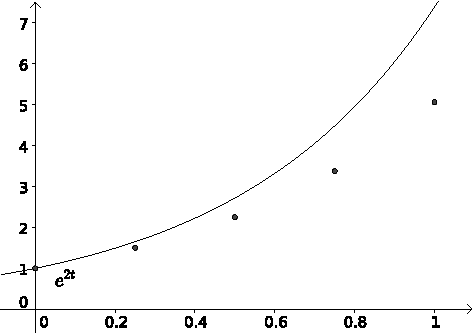
\includegraphics{figures/ode-pendulum02}
\end{figure}
Lihat Gambar \ref{fig:odeApproxSolution}. Aproksimasi tersebut baik
untuk nilai $t$ yang mendekati nol, tetapi kurang baik untuk nilai
$t$ yang mendekati 1. 

\subsection{Masalah Nilai Awal\index{masalah nilai awal}}

Seperti persamaan aljabar, persamaan diferensial dapat memiliki lebih
dari satu solusi. Kita telah melihat bahwa $\theta=e^{2t}$ merupakan
solusi dari $3\ddot{\theta}-8\dot{\theta}+4\theta=0$. Demikian pula
$\theta=5e^{2t}$, $\theta=-2.1e^{2t}$, dan $\theta=\sqrt{7\pi}e^{2t}$.
Bahkan, $\theta=ce^{2t}$ merupakan solusi untuk sembarang konstanta
$c$. PDB $3\ddot{\theta}-8\dot{\theta}+4\theta=0$ memiliki tak terhingga
banyak solusi! Verifikasinya merupakan latihan sederhana. Untuk $\theta=ce^{2t}$,
$\dot{\theta}=2ce^{2t}$ dan $\ddot{\theta}=4ce^{2t}$, sehingga
\begin{eqnarray*}
3\ddot{\theta}-8\dot{\theta}+4\theta & = & 3(4ce^{2t})-8(2ce^{2t})+4(ce^{2t})\\
 & = & 12c(e^{2t})-16c(e^{2t})+4c(e^{2t})\\
 & = & (12c-16c+4c)e^{2t}\\
 & = & 0.
\end{eqnarray*}
Selain itu, $\theta=ae^{2t/3}$ merupakan solusi untuk sembarang konstanta
$a$. Solusi ini dapat diverifikasi dengan cara yang sama seperti
solusi $\theta=ce^{2t}$ diverifikasi. Dapatkah Anda melakukannya?
Jawaban \vpageref{odeMoreSolutions}. Terakhir, $\theta=ce^{2t}+ae^{2t/3}$
juga merupakan solusi untuk sembarang pasangan konstanta $c$ dan
$a$! Dapatkah Anda membuktikannya? Jawaban \vpageref{odeEvenMoreSolutions}.
Tidak jarang sebuah persamaan diferensial memiliki tak terhingga banyak
solusi. 

Persamaan diferensial lain yang memiliki tak terhingga banyak solusi
adalah 
\[
\dot{y}=\frac{t}{y}.
\]
Solusinya adalah $y=\sqrt{t^{2}+c}$ dan $y=-\sqrt{t^{2}+a}$, yang
berlaku untuk sembarang konstanta $c$ dan $a$ selama $y\neq0$.
Solusi kompleks diperbolehkan! Namun, jika kita juga mensyaratkan
$y(0)=1$, hanya ada satu solusi! $y=-\sqrt{t^{2}+c}$ bukan lagi
solusi karena memberikan nilai negatif bagi $y$ untuk semua nilai
$t$. Adapun $y=\sqrt{t^{2}+c}$ hanya merupakan solusi jika $c=1$.
Solusi \textit{satu-satunya} adalah $y=\sqrt{t^{2}+1}$. 

Syarat $y(0)=1$ disebut nilai awal, atau kondisi awal, dan pasangan
persamaan
\begin{eqnarray*}
\dot{y} & = & \frac{t}{y}\\
y(0) & = & 1
\end{eqnarray*}
 disebut masalah nilai awal. Secara lebih umum, pasangan persamaan
\begin{eqnarray*}
\dot{y} & = & f(y,t)\\
y(t_{0}) & = & y_{0}
\end{eqnarray*}
membentuk apa yang dikenal sebagai masalah nilai awal orde pertama.\index{masalah nilai awal}

\noindent\begin{digression}{Terdapat tepat satu solusi dari $\dot y=\frac{t}{y}$ yang memenuhi $y(0)=1$.}

\noindent Dengan menetapkan $y=\sqrt{t^{2}+1}$, diperoleh $\dot{y}=\frac{1}{2}\frac{1}{\sqrt{t^{2}+1}}(2t)=\frac{t}{\sqrt{t^{2}+1}}$.
Dengan demikian, persamaan $\dot{y}=\frac{t}{y}$ menjadi
\[
\frac{t}{\sqrt{t^{2}+1}}=\frac{t}{\sqrt{t^{2}+1}},
\]
suatu pernyataan yang tak dapat disangkal kebenarannya. Oleh karena
itu, $y=\sqrt{t^{2}+1}$ merupakan solusi dari $\dot{y}=\frac{t}{y}$.
Selain itu, $y(0)=\sqrt{0^{2}+1}=1$, sehingga solusi khusus $y=\sqrt{t^{2}+1}$
juga memenuhi syarat $y(0)=1$. Dengan demikian, $y=\sqrt{t^{2}+1}$
merupakan \textit{salah satu} solusi---dan satu-satunya solusi yang
berbentuk $y=\sqrt{t^{2}+c}$ atau $y=-\sqrt{t^{2}+a}$. Namun, apakah
fungsi tersebut merupakan \textit{satu-satunya} solusi dalam bentuk
apa pun? Mungkin ada fungsi lain yang memenuhi persamaan diferensial
tersebut. Sedikit kalkulus seharusnya membantu menyelesaikan persoalan
ini. Inti pembuktian ini adalah menunjukkan bahwa $y=\sqrt{t^{2}+c}$
dan $y=-\sqrt{t^{2}+a}$ merupakan \textit{satu-satunya} solusi dari
$\dot{y}=\frac{t}{y}$. Rangkaian persamaan berikut menunjukkannya.
Setiap baris menyiratkan baris berikutnya. 
\begin{eqnarray*}
\frac{dy}{dt} & = & \frac{t}{y},\qquad y\neq0\\
y\,dy & = & t\,dt,\qquad y\neq0\\
\int y\,dy & = & C+\int t\:dt,\qquad y\neq0\\
\frac{1}{2}y^{2} & = & C+\frac{1}{2}t^{2},\qquad y\neq0\\
y^{2} & = & 2C+t^{2},\qquad y\neq0\\
y & = & \pm\sqrt{t^{2}+2C},\qquad y\neq0.
\end{eqnarray*}
Mengganti konstanta $2C$ dengan $c$ atau $a$ tidak mengubah fakta
bahwa suku tersebut merupakan konstanta sembarang, sehingga $y=\sqrt{t^{2}+c}$
dan $y=-\sqrt{t^{2}+a}$ merupakan satu-satunya solusi dari $\dot{y}=\frac{t}{y}$.
Metode penyelesaian persamaan diferensial ini disebut pemisahan variabel\index{pemisahan variabel}.

\noindent\end{digression}

\subsection{Konsep Utama}
\begin{description}
\item [{Solusi\ aproksimasi\ bagi\ suatu\ persamaan\ diferensial:}] sekumpulan
titik yang, idealnya, terletak di dekat grafik suatu solusi eksak.
\item [{Derajat\ dari\ suatu\ persamaan\ diferensial:}] sama dengan
orde turunan tertinggi yang muncul dalam persamaan tersebut.
\item [{Persamaan\ diferensial:}] persamaan yang memuat turunan (atau
diferensial).
\item [{Diagram\ benda\ bebas:}] suatu diagram teknik yang hanya terdiri
atas sebuah benda dan gaya-gaya yang bekerja padanya.
\item [{Masalah\ nilai\ awal:}] persamaan diferensial yang dilengkapi
dengan suatu nilai solusi yang disyaratkan.
\item [{Hukum\ gerak\ kedua\ Newton:\ percepatan}] suatu benda berbanding
lurus dengan besar gaya resultan yang diberikan pada benda tersebut,
searah dengan gaya resultan, dan berbanding terbalik dengan massa
benda---sering diringkas dengan persamaan $F=ma$. Persamaan ini
mengasumsikan bahwa massa benda konstan.
\item [{Persamaan\ diferensial\ biasa\ (PDB):}] persamaan diferensial
yang hanya memiliki satu variabel bebas.
\item [{Solusi\ dari\ suatu\ persamaan\ diferensial:}] fungsi yang,
ketika disubstitusikan untuk variabel terikat, membuat persamaan tersebut
menjadi pernyataan yang benar.
\end{description}
\startexercises 

\subsection{Latihan}
\begin{enumerate}
\item Nyatakan derajat persamaan diferensial tersebut.

\begin{enumerate}
\item \label{exc:odePendulum}$\dot{y}=y$ \hasananswer 
\item $y''=6x+\sin x$
\item \label{exc:odePendulum-1}$\ddot{s}+\dot{s}+s=0$ \hasananswer 
\item \label{exc:odePendulum-2}$f'+\frac{f}{x}=x^{2}$ \hasasolution 
\item $(2h+x)h'+h=4x$
\item \label{exc:odePendulum-3}$\ddot{r}\dot{r}t^{2}=-\frac{1}{8}$ \hasananswer 
\end{enumerate}
\item Verifikasi bahwa fungsi tersebut merupakan solusi persamaan diferensial.

\begin{enumerate}
\item \label{exc:odePendulum-4}$y(t)=e^{t}$; $\dot{y}=y$ \hasananswer 
\item $y(x)=x^{3}-26.83x-\sin x$; $y''=6x+\sin x$
\item \label{exc:odePendulum-5}$s(t)=e^{-t/2}\sin\left(\frac{\sqrt{3}}{2}t\right)$;
$\ddot{s}+\dot{s}+s=0$ \hasananswer 
\item \label{exc:odePendulum-6}$f(x)=\frac{x^{3}}{4}+\frac{4}{x}$, $x>0$;
$f'+\frac{f}{x}=x^{2}$ \hasasolution 
\item $h(x)=-2x$; $(2h+x)h'+h=4x$
\item \label{exc:odePendulum-7}$r(t)=\sqrt{t}$, $t>0$; $\ddot{r}\dot{r}t^{2}=-\frac{1}{8}$ \hasananswer 
\end{enumerate}
\item Verifikasi bahwa fungsi tersebut merupakan solusi masalah nilai awal.

\begin{enumerate}
\item \label{exc:odePendulum-8}$y(t)=4e^{t}$; $\dot{y}=y$, $y(0)=4$ \hasananswer 
\item $y(x)=x^{3}-\sin x-\pi^{3}$; $y'=3x^{2}-\cos x$, $y(\pi)=0$
\item \label{exc:odePendulum-9}$s(t)=\frac{1}{2}\left(1+e^{-t^{2}}\right)$;
$\dot{s}=(1-2s)t$, $s(0)=1$ \hasananswer 
\item \label{exc:odePendulum-10}$f(x)=\frac{x^{3}}{4}+\frac{16}{x}$, $x>0$;
$f'=-\frac{f}{x}+x^{2}$, $f(4)=20$ \hasasolution 
\item $h(x)=-2x-1$; $h'=\frac{1+4x-h}{2h+x+1}$, $h(0)=-1$
\item \label{exc:odePendulum-11}$r(t)=\sqrt{t}-3$, $t>0$; $\ddot{r}\dot{r}t^{2}=-\frac{1}{8}$,
$r(9)=0$, $\dot{r}(9)=\frac{1}{6}$. \hasananswer  PETUNJUK: Solusi
harus memenuhi PDB tersebut dan kedua syarat, $r(9)=0$ dan $\dot{r}(9)=\frac{1}{6}$.
\end{enumerate}
\item Selesaikan persamaan diferensial tersebut.

\begin{enumerate}
\item \label{exc:odePendulum-12}$y'=5x^{4}$ \hasananswer 
\item $y'=3xe^{x^{2}}$
\item \label{exc:odePendulum-13}$\dot{y}=t-\sin t$ \hasasolution 
\item \label{exc:odePendulum-14}$\dot{y}=\frac{1}{t}$, $t<0$ \hasananswer 
\item $s'=1-\ln x$
\item \label{exc:odePendulum-15}$\dot{s}=3te^{t}$ \hasananswer 
\end{enumerate}
\item Diberikan suatu masalah nilai awal, solusi eksaknya, dan suatu solusi
aproksimasi. Berikan komentar mengenai seberapa baik solusi aproksimasi
tersebut menghampiri solusi eksak.

\begin{enumerate}
\item \label{exc:odePendulum-16}$\dot{y}=y$, $y(0)=4$; $y(t)=4e^{t}$;
$\{(0,4),(.25,5),(.5,6.3),(.75,7.8),(1,9.8)\}$ \hasananswer 
\item $y'=3x^{2}-\cos x$, $y(\pi)=0$; $y(x)=x^{3}-\sin x-\pi^{3}$; $\{(\pi,0),(\frac{5}{4}\pi,30),(\frac{3}{2}\pi,74),(\frac{7}{4}\pi,135),(2\pi,216)\}$
\item \label{exc:odePendulum-17}$\dot{s}=(1-2s)t$, $s(0)=1$; $s(t)=\frac{1}{2}\left(1+e^{-t^{2}}\right)$;
$\{(0,1),(.5,1),(1,.75),(1.5,.5),(2,.5)\}$ \hasananswer 
\item \label{exc:odePendulum-18}$f'=-\frac{f}{x}+x^{2}$, $f(4)=20$; $f(x)=\frac{x^{3}}{4}+\frac{16}{x}$;
$\{(4,20),(4.25,23),(4.5,26),(4.75,30),(5,34)\}$ \hasasolution 
\item $h'=\frac{1+4x-h}{2h+x+1}$, $h(0)=-1$; $h(x)=-2x-1$; $\{(0,-1),(.25,-1.5),(.5,-2),(.75,-2.5),(1,-3)\}$
\item \label{exc:odePendulum-19}$\ddot{r}\dot{r}t^{2}=-\frac{1}{8}$, $r(9)=0$,
$\dot{r}(9)=-\frac{1}{6}$; $r(t)=\sqrt{t}-3$; $\{(9,0),(10,.16),(11,.31),(12,.46),(13,.61)\}$
 \hasananswer 
\end{enumerate}
\item \label{exc:fbd}Gambarlah diagram benda bebas untuk situasi tersebut.

\begin{enumerate}
\item \label{exc:odePendulum-20}\label{dom-start}Gerak bandul dengan mengabaikan
hambatan udara (tanpa redaman). \hasananswer 
\item \label{exc:odePendulum-21}Sebuah balok yang meluncur menuruni bidang
miring. \hasananswer 
\item \label{exc:odePendulum-22}Sebuah balok yang diam di atas bidang miring
(tidak bergerak). \hasasolution 
\item Sebuah balok yang didorong menaiki bidang miring.
\item \label{exc:odePendulum-23}Sebuah sofa yang didorong melintasi lantai
datar dengan gaya terapan yang sejajar dengan lantai. \hasananswer 
\item \label{exc:odePendulum-24}Sebuah sofa yang didorong melintasi lantai
datar dengan gaya terapan yang tidak sejajar dengan lantai. \hasasolution 
\item \label{exc:odePendulum-25}Sebuah sofa yang didorong ke atas pada
lantai kayu keras tua yang miring. Gaya terapan dapat sejajar ataupun
tidak sejajar dengan lantai. \hasananswer 
\item \label{exc:odePendulum-26}Seorang pengendara kereta luncur telah
mencapai kaki bukit (dan sekarang bergerak di atas salju yang datar)
lalu meluncur tanpa dorongan hingga berhenti. \hasananswer 
\item \label{exc:odePendulum-27}Seorang pengendara kereta luncur yang sedang
meluncur menuruni bukit. \hasananswer 
\item \label{exc:odePendulum-28}Sebuah keping hoki yang meluncur melintasi
gelanggang es. \hasananswer 
\item \label{dom-end}Sebuah keping hoki yang meluncur di atas es dengan
kelajuan konstan (dengan mengabaikan gesekan).
\item \label{exc:odePendulum-29}\label{vert-start}Seorang penerjun payung
yang sedang jatuh. \hasananswer 
\item \label{exc:odePendulum-30}Seorang penerjun payung yang parasutnya
baru saja terbuka. \hasasolution 
\item \label{exc:odePendulum-31}Seorang penerjun payung yang parasutnya
baru saja terbuka sementara angin sepoi-sepoi yang tetap bertiup ke
samping. \hasananswer 
\item \label{exc:odePendulum-32}Sebuah bola sepak yang semula ditendang
pada sudut 40 derajat dan kini tepat mencapai titik tertingginya,
dengan hambatan udara diabaikan. \hasananswer 
\item \label{vert-end}Sebuah bola sepak yang bergerak naik dan ke kanan
saat mendekati titik tertingginya, dengan hambatan udara diabaikan.
\end{enumerate}
\item \label{exc:odePendulum-34}Gunakan diagram benda bebas dari soal \ref{exc:fbd}
untuk menentukan persamaan gerak dalam arah tangensial untuk (\ref{dom-start})-(\ref{dom-end}),
dan dalam arah vertikal untuk (\ref{vert-start})-(\ref{vert-end}). \haspartwithsolution  \haspartwithanswer 
\item \label{exc:odePendulum-33}Seberapa jauh lebih mudah menggeser sofa
dengan mendorongnya sejajar dengan lantai dibandingkan dengan mendorongnya
sedikit ke arah lantai? Bandingkan gesekan kinetik pada sofa yang
didorong sejajar dengan lantai dengan sofa yang didorong membentuk
sudut 20 derajat dari arah sejajar dengan lantai. Kemudian hitung
gaya terapan yang diperlukan untuk mengatasi gesekan kinetik dalam
setiap kasus. Anggap lantainya datar. \hasananswer 
\end{enumerate}
\finishexercises 

\subsection*{Jawaban}
\begin{description}
\item [{\label{odeMoreSolutions}$\theta=ae^{2t/3}$\ merupakan\ suatu\ solusi\ dari}] $3\ddot{\theta}-8\dot{\theta}+4\theta=0$:
$\dot{\theta}=\frac{2}{3}ae^{2t/3}$ dan $\ddot{\theta}=\frac{4}{9}ae^{2t/3}$
sehingga 
\begin{eqnarray*}
3\ddot{\theta}-8\dot{\theta}+4\theta & = & 3\left(\frac{4}{9}ae^{2t/3}\right)-8\left(\frac{2}{3}ae^{2t/3}\right)+4\left(ae^{2t/3}\right)\\
 & = & \frac{4}{3}a(e^{2t/3})-\frac{16}{3}a(e^{2t/3})+\frac{12}{3}a(e^{2t/3})\\
 & = & \left(\frac{4}{3}a-\frac{16}{3}a+\frac{12}{3}a\right)e^{2t/3}\\
 & = & 0.
\end{eqnarray*}
\item [{\label{odeEvenMoreSolutions}$\theta=ce^{2t}+ae^{2t/3}$\ merupakan\ suatu\ solusi\ dari\ $3\ddot{\theta}-8\dot{\theta}+4\theta=0$:}] $\dot{\theta}=2ce^{2t}+\frac{2}{3}ae^{2t/3}$
dan $\ddot{\theta}=4ce^{2t}+\frac{4}{9}ae^{2t/3}$ sehingga 
\begin{eqnarray*}
3\ddot{\theta}-8\dot{\theta}+4\theta & = & 3\left(4ce^{2t}+\frac{4}{9}ae^{2t/3}\right)-8\left(2ce^{2t}+\frac{2}{3}ae^{2t/3}\right)+4\left(ce^{2t}+ae^{2t/3}\right)\\
 & = & 12c(e^{2t})+\frac{4}{3}a(e^{2t/3})-16c(e^{2t})-\frac{16}{3}a(e^{2t/3})+4c(e^{2t})+\frac{12}{3}a(e^{2t/3})\\
 & = & (12c-16c+4c)e^{2t}+\left(\frac{4}{3}a-\frac{16}{3}a+\frac{12}{3}a\right)e^{2t/3}\\
 & = & 0.
\end{eqnarray*}
\end{description}

